\documentclass[
    17pt,
    margin=1in,
    innermargin=-4.5in,
    blockverticalspace=-0.15in
]{tikzposter}
\geometry{paperwidth=42in,paperheight=30in}
\usepackage[utf8]{inputenc}
\usepackage{amsmath}
\usepackage{amsfonts}
\usepackage{amsthm}
\usepackage{amssymb}
\usepackage{mathrsfs}
\usepackage{graphicx}
\usepackage{subcaption}
\usepackage{adjustbox}
\usepackage{enumitem}
\usepackage{multirow}
\usepackage[backend=biber,style=apa]{biblatex}
\usepackage{emory-theme}
\usepackage{inconsolata} % very nice fixed-width font included with texlive-full
\usepackage{color} % more flexible names for syntax highlighting colors
\usepackage{listings}
\lstdefinelanguage{julia}
{
  keywordsprefix=\@,
  morekeywords={
    exit,whos,edit,load,is,isa,isequal,typeof,tuple,ntuple,uid,hash,finalizer,convert,promote,
    subtype,typemin,typemax,realmin,realmax,sizeof,eps,promote_type,method_exists,applicable,
    invoke,dlopen,dlsym,system,error,throw,assert,new,Inf,Nan,pi,im,begin,while,for,in,return,
    break,continue,macro,quote,let,if,elseif,else,try,catch,end,bitstype,ccall,do,using,module,
    import,export,importall,baremodule,immutable,local,global,const,Bool,Int,Int8,Int16,Int32,
    Int64,Uint,Uint8,Uint16,Uint32,Uint64,Float32,Float64,Complex64,Complex128,Any,Nothing,None,
    function,type,typealias,abstract
  },
  sensitive=true,
  morecomment=[l]{\#},
  morestring=[b]',
  morestring=[b]" 
}

\definecolor{mygray}{RGB}{128,128,128}
\definecolor{myblue}{RGB}{0, 0, 255}
\definecolor{myolivegreen}{RGB}{186, 184, 108}
\definecolor{mymaroon}{RGB}{128, 0, 0}

\lstset{
    language=julia,
    basicstyle=\ttfamily, 
    columns=fullflexible, % make sure to use fixed-width font, CM typewriter is NOT fixed width
    numbers=left, 
    numberstyle=\small\ttfamily\color{mygray},
    stepnumber=1,              
    numbersep=10pt, 
    numberfirstline=true, 
    numberblanklines=true, 
    tabsize=4,
    lineskip=-1.5pt,
    extendedchars=true,
    breaklines=true,        
    keywordstyle=\color{myblue}\bfseries,
    identifierstyle=, % using emph or index keywords
    commentstyle=\sffamily\color{myolivegreen},
    stringstyle=\color{mymaroon},
    showstringspaces=false,
    showtabs=false,
    upquote=false
}

\usepackage{mwe}    % for placeholder images

\addbibresource{refs.bib}

% Set theme parameters
\tikzposterlatexaffectionproofoff
\usetheme{EmoryTheme}
\usecolorstyle{EmoryStyle}

\title{AdvancedHMC.jl: a modular implementation of Stan’s no-U-turn sampler in Julia}
\author{Kai Xu\textsuperscript{1}, Hong Ge\textsuperscript{2}, Will Tebbutt\textsuperscript{2} and Mohamed Tarek\textsuperscript{3}}
\institute{
    \textsuperscript{1}University of Edinburgh, United Kingdom \quad \textsuperscript{2}University of Cambridge, United Kingdom \quad \textsuperscript{3}UNSW Canberra, Australia
}
\titlegraphic{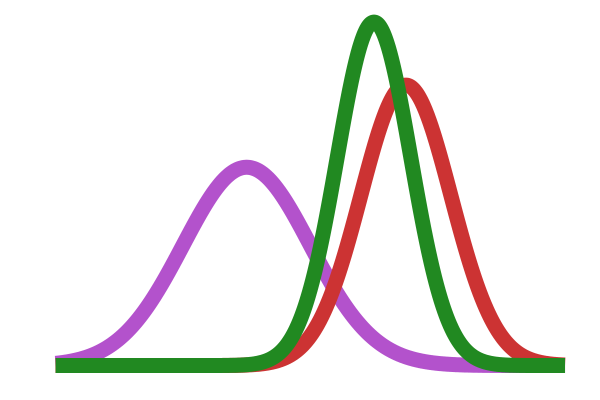
\includegraphics[width=0.075\textwidth]{turing-logo}}

% begin document
\begin{document}
\maketitle
\centering
\begin{columns}

\column{0.32}

\block{Abstract}{
    The No-U-Turn Sampler (NUTS) in Stan has demonstrated remarkable sampling robustness and 
    efficiency in a wide range of Bayesian inference problems, 
    due to the use of self-adaptive Hamiltonian dynamic trajectory simulation length, 
    together with a fine-tuned joint adaptation of step-size and mass matrix. 
    Motivated by these successes, we present 
    AdvancedHMC.jl: a pure Julia implementation of Stan’s built-in NUTS and 
    related adaptation methods. 
    We hope AdvancedHMC.jl can expose Stan’s NUTS to a wider range of users, 
    e.g. those who want to write their models by hand, 
    or using a different probabilistic programming language (e.g. Turing, Soss). 
    In our package, NUTS is defined as a combination of individual components with 
    abstractions 
%  including the `Hamiltonian` dynamics, the `Metric` space, 
%  how the dynamics are numerically simulated by an Integrator to build up a `Trajectory`, 
%  and how a candidate point is sampled from it by a `TrajectorySampler`. 
%  This abstraction is partially 
    inspired by 
    (\cite{betancourt2017conceptual}).
    % A Conceptual Introduction to Hamiltonian Monte Carlo” by Michael Betancourt.
}

\block{Hamiltonian Monte Carlo Components}{
    AdvancedHMC supports the following combination of different HMC samplers.
    $$
    (\{FixedStepSizeHMC, FixedLengthHMC\} \cup DynamicHMC) \circ Adaptor.
    $$
    Here $DynamicHMC$ are a combination of different NUTS components
    $$
    Metric \times Integrator \times TrajectorySampler \times TerminationCriterion,
    $$
    where 
    \begin{equation*}
        \begin{aligned} 
            Metric &=  \{ UnitEuclidean, DiagEuclidean, DenseEuclidean \} \\ 
            Integrator &=  \{ Leapfrog \} \\
            TrajectorySampler &=  \{ Slice, Multinomial \} \\
            TerminationCriterion &= \{ ClassicNoUTurn, GeneralisedNoUTurn \}
        \end{aligned}
    \end{equation*}
    and $Adaptor$ is a compositional adaptor composed from base adaptors
    $$
    BaseAdaptor \in \{Preconditioner, NesterovDualAveraging\}.
    $$

    \textbf{Note 1}: $Preconditioner$ behaves corresponding to the choice of metric spaces.

    \textbf{Note 2}: a specific composition called $StanHMCAdaptor$ is provided to construct Stan's windowed adaptor, 
    which is proved to be robust in practice.
}

\block{Benchmark Models}{
    We use five models from MCMCBenchmarks.jl to compare 
    NUTS between AdvancedHMC.jl and Stan.
    \paragraph{Gaussian Model (Gaussian)}
    is a simple two parameter Gaussian distribution.
    $$
    \mu \sim \mathcal{N}(0, 1), \quad 
    \sigma \sim \mathcal{T}runcated(\mathcal{C}auchy(0, 5), 0, \infty), \quad
    y_n \sim \mathcal{N}(\mu, \sigma) \; (n = 1, \dots, N)
    $$
    \paragraph{Signal Detection Model (SDT)}
    is a simple model used in psychophysics and signal processing, 
    which decomposes performance in terms of discriminability and bias.
    $$
    d \sim \mathcal{N}(0, \frac{1}{\sqrt{2}}), \quad 
    c \sim \mathcal{N}(0, \frac{1}{\sqrt{2}}), \quad 
    x \sim \text{SDT}(d, c)
    $$
    \paragraph{Linear Regression Model (LR)}
    $$
    B_d \sim \mathcal{N}(0, 10), \;
    \sigma \sim \mathcal{T}runcated(\mathcal{C}auchy(0, 5), 0, \infty), \;
    y_n \sim \mathcal{N}(\mu_n, \sigma),
    $$
    where $\mu = B_0 + B^T X, d = 1, \dots, D$ and $n = 1, \dots, N$.
    \paragraph{Hierarchical Poisson Regression (HPR)}
    $$
    a_0 \sim \mathcal{N}(0, 10), \;
    a_1 \sim \mathcal{N}(0, 1), \;
    b_\sigma \sim \mathcal{T}runcated(\mathcal{C}auchy(0, 1), 0, \infty), \;
    b_d \sim \mathcal{N}(0, b_\sigma), \;
    y_n \sim \mathcal{P}(\lambda_n),
    $$
    where $\lambda_n = \exp(a_0 + b_{z_n} + a_1 x_n), d = 1, \dots, N_b$ and $n = 1, \dots, N$.
    \paragraph{Linear Ballistic Accumulator (LBA)}
    is a cognitive model of perception and simple decision making.
    $$
    \tau \sim \mathcal{T}runcated(\mathcal{N}(0.4, 0.1), 0, mn), \quad
    A \sim \mathcal{T}runcated(\mathcal{N}(0.8, 0.4), 0, \infty),
    $$
    $$
    k \sim \mathcal{T}runcated(\mathcal{N}(0.2, 0.3), 0, \infty), \quad
    \nu_d \sim \mathcal{N}(0, 3), \quad
    x_i \sim \text{LBA}(\nu, \tau, A, k)
    $$
    where $mn=\min_i x_{i,2}, d = 1, \dots, N_c$ and $i = 1, \dots, N$.
}

\column{0.36}

\block{Example Code of Building Stan's NUTS}{
    \lstinputlisting{example.jl}
}

\block{Inference Results}{
    To compare the inference results between AHMC and Stan,
    we run multiple runs of NUTS of targt acceptance rate $0.8$ 
    for $2,000$ runs with $1,000$ adaptation steps,
    where the warm-up samples dropped out.
    Below are figures of distributions of step size and tree depth,
    as well as the averaged effective sample size (ESS) for different variables.
    \begin{tikzfigure}[Gaussian (50 runs); left to right: step size, tree depth, ESS]
        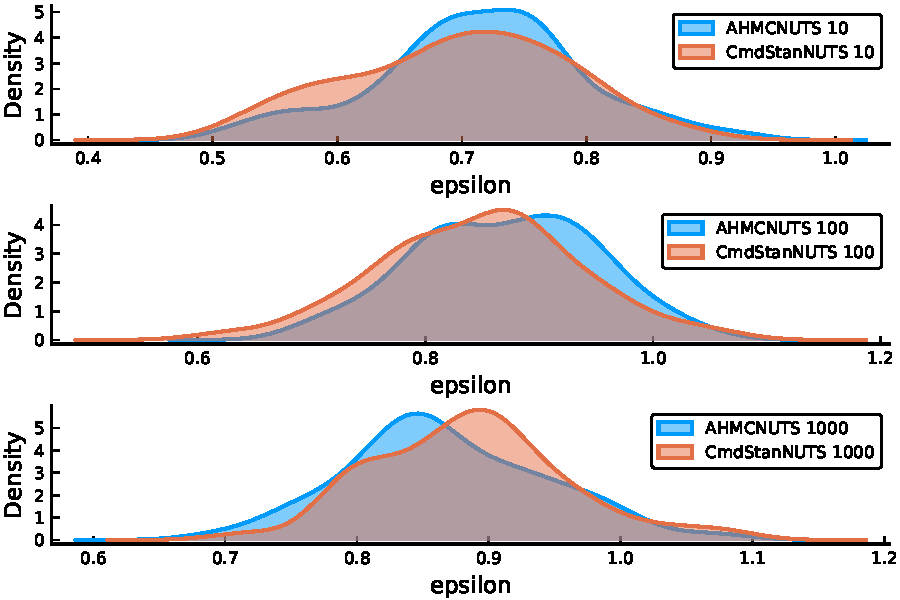
\includegraphics[width=0.08\textwidth]{./figs/Gaussian/density_epsilon.pdf}
        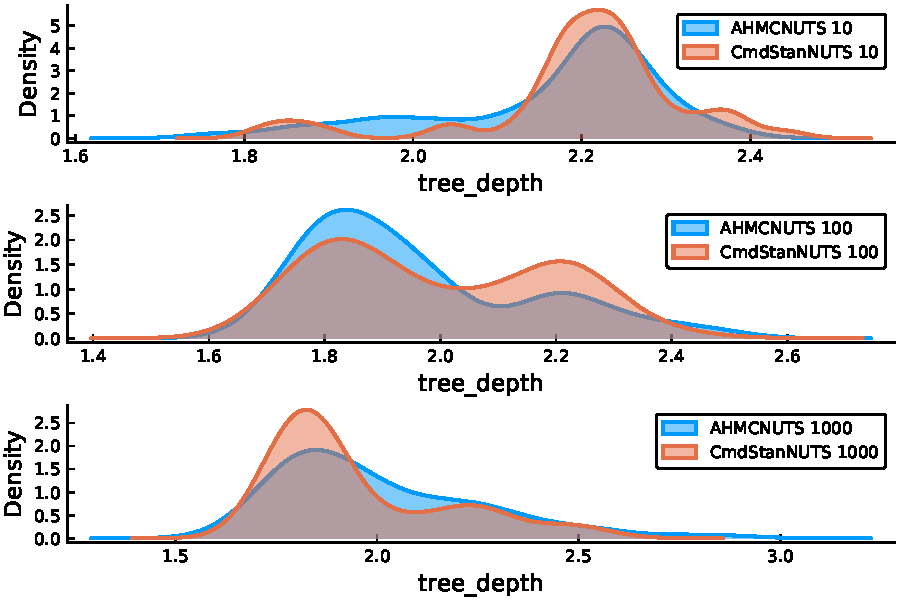
\includegraphics[width=0.08\textwidth]{./figs/Gaussian/density_tree_depth.pdf}
        \raisebox{\height}{\scalebox{0.75}{
            \begin{tabular}{llll}
                \multirow{2}{*}{Sampler} & \multirow{2}{*}{$N$} & \multicolumn{2}{c}{ESS} \\
                & & $\mu$ & $\sigma$ \\
                \hline \\
                Stan & 10 & 513.163 & 466.577 \\
                AHMC & 10 & 503.535 & 447.722 \\
                Stan & 100 & 786.531 & 782.231 \\
                AHMC & 100 & 786.531 & 796.628 \\
                Stan & 1000 & 864.01 & 876.66 \\
                AHMC & 1000 & 832.255 & 844.452 \\
            \end{tabular}
        }}
    \end{tikzfigure}
    \begin{tikzfigure}[SDT (100 runs); left to right: step size, tree depth, ESS]
        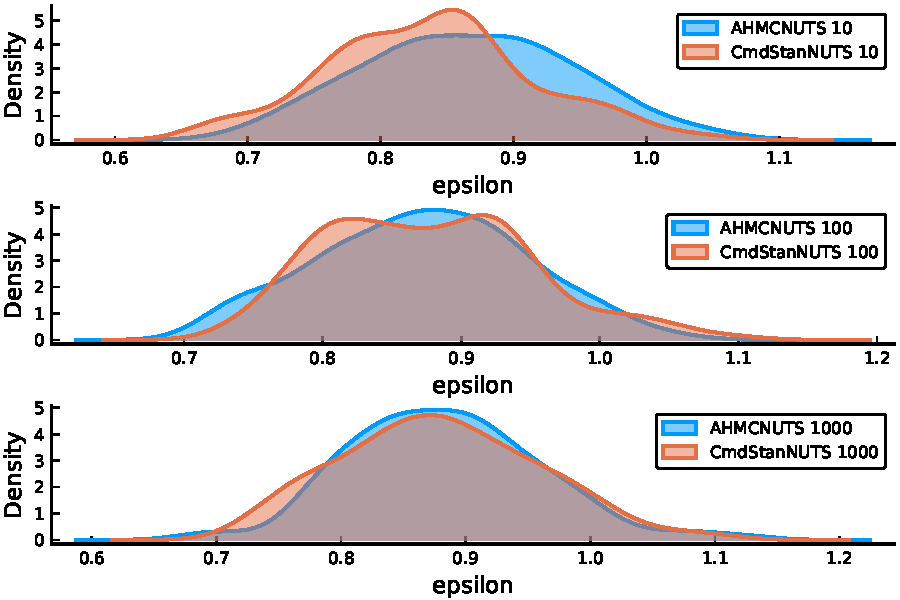
\includegraphics[width=0.08\textwidth]{./figs/SDT/density_epsilon.pdf}
        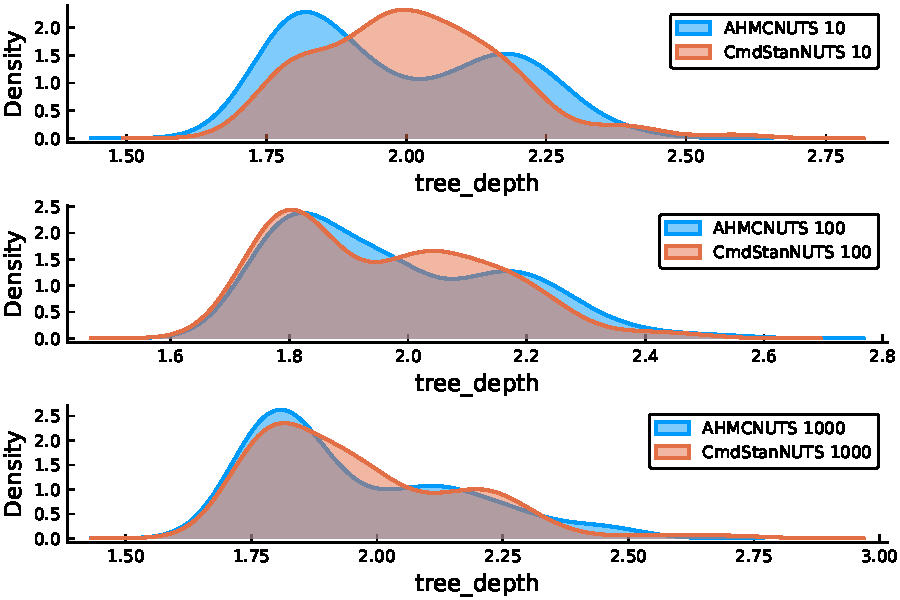
\includegraphics[width=0.08\textwidth]{./figs/SDT/density_tree_depth.pdf}
        \raisebox{\height}{\scalebox{0.75}{
            \begin{tabular}{llll}
                \multirow{2}{*}{Sampler} & \multirow{2}{*}{$N$} & \multicolumn{2}{c}{ESS} \\
                & & $d$ & $c$ \\
                \hline \\
                Stan & 10 & 710.762  & 703.327 \\
                AHMC & 10 & 802.236 & 815.929 \\
                Stan & 100 & 820.741 & 823.152 \\
                AHMC & 100 & 814.308 & 846.357 \\
                Stan & 1000 & 844.478 & 872.961 \\
                AHMC & 1000 & 829.792 & 859.018 \\
            \end{tabular}
        }}
    \end{tikzfigure}
    \begin{tikzfigure}[LR (50 runs); left to right: step size, tree depth, ESS]
        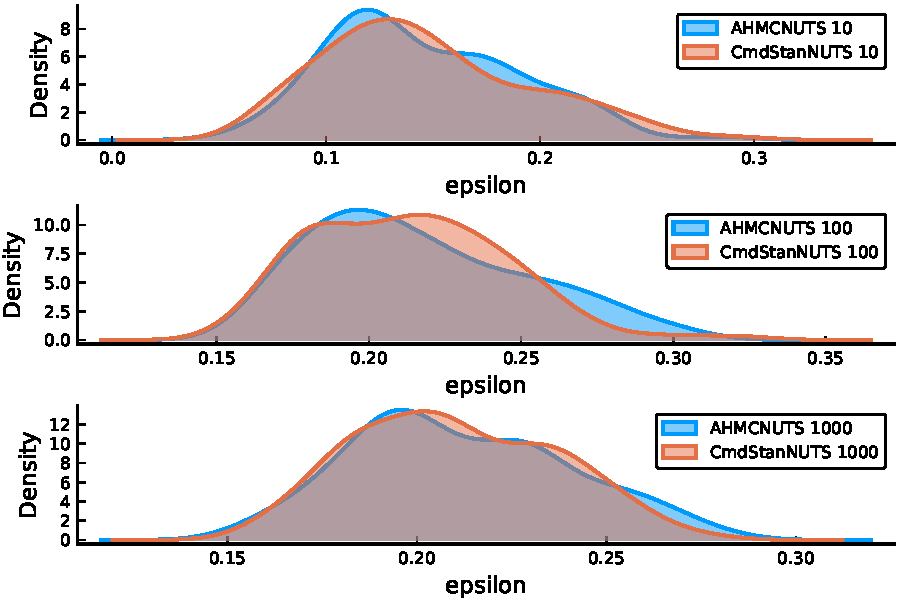
\includegraphics[width=0.08\textwidth]{./figs/Linear_Regression/density_epsilon.pdf}
        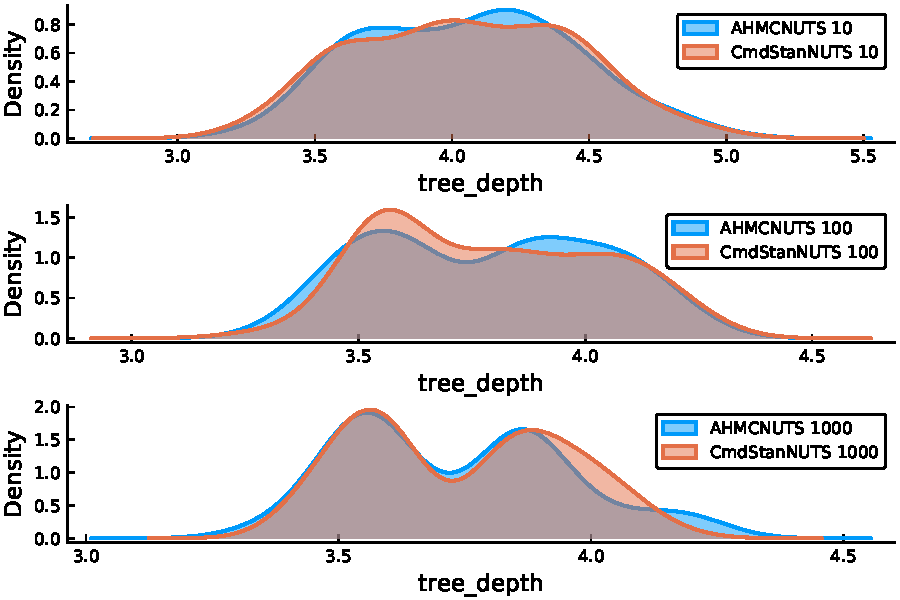
\includegraphics[width=0.08\textwidth]{./figs/Linear_Regression/density_tree_depth.pdf}
        \raisebox{\height}{\scalebox{0.75}{
            \begin{tabular}{llllll}
                \multirow{2}{*}{Sampler} & \multirow{2}{*}{$N$} & \multicolumn{4}{c}{ESS} \\
                & & $b_0$ & $\sigma$ & $b_1$ & $b_2$ \\
                \hline \\
                Stan & 10 & 413.939 & 266.476 & 381.219 & 423.441 \\
                AHMC & 10 & 354.946 & 263.894 & 411.769 & 399.42 \\
                Stan & 100 & 621.796 & 729.812 & 465.99 & 608.608 \\
                AHMC & 100 & 473.005 & 734.189 & 606.996 & 621.543 \\
                Stan & 1000 & 668.524 & 789.987 & 464.459 & 648.201 \\
                AHMC & 1000 & 485.988 & 786.577 & 676.097 & 689.344 \\
            \end{tabular}
        }}
    \end{tikzfigure}
}

\column{0.32}
\block{Performance}{
    Put plots for performance.
}

\block{Remarks}{
    CuArrays.jl

    Bijectors.jl
}

\block{Acknowledgements}{
    We would like to thank the developers of MCMCBenchmarks.jl, Rob Goedman and Christopher Fisher.
    With this package we run all the benchmarks and generate all the plots used in this poster.
}

\block{References}{
    \vspace{-1em}
    \printbibliography[heading=none]
}
    
\end{columns}
\end{document}